\documentclass[10pt,twoside,a4paper,titlepage]{article}
\linespread{1.3}
\usepackage{indentfirst}
\usepackage{amsmath}
\usepackage{graphicx}
\usepackage{fancyhdr}
\usepackage{setspace}
\usepackage[UTF8]{ctex}

\title{EE101 Final Project Report}
\author{Yifu Chen,Jialong Guo , Ziliang Guo, Aofan Jiang}

\begin{document}

\maketitle
\phantom{s}
\thispagestyle{empty}
\clearpage

\tableofcontents
\thispagestyle{empty}
\newpage
\setcounter{page}{1}

\section{Overview}
\subsection{Project File Tree}
	% \includegraphics[width=0.7\textwidth]{pics/01.jpg}

\subsection{Develop Environment}


	% Windows 8.1\par
	% XAMPP Version 7.3.2\par
	% MySQL Ver 15.1 Distrib 10.1.38-MariaDB, for Win64 (AMD64)\par
	% Solr 8.0.0\par
	% Browser Google Chrome 74.0.3729.157
	% Editor Sublime Text Version 3.2.1 Build 3027\par
\section{Front-end}
written by Yifu Chen
	%cyf's part
	
	I was in charge of the front-end part.I mainly used CSS and BOOTSTRAP to beauify our websitek,and I will introduce my work  of each page respectively.
	
	\subsection{Index.php}
	
	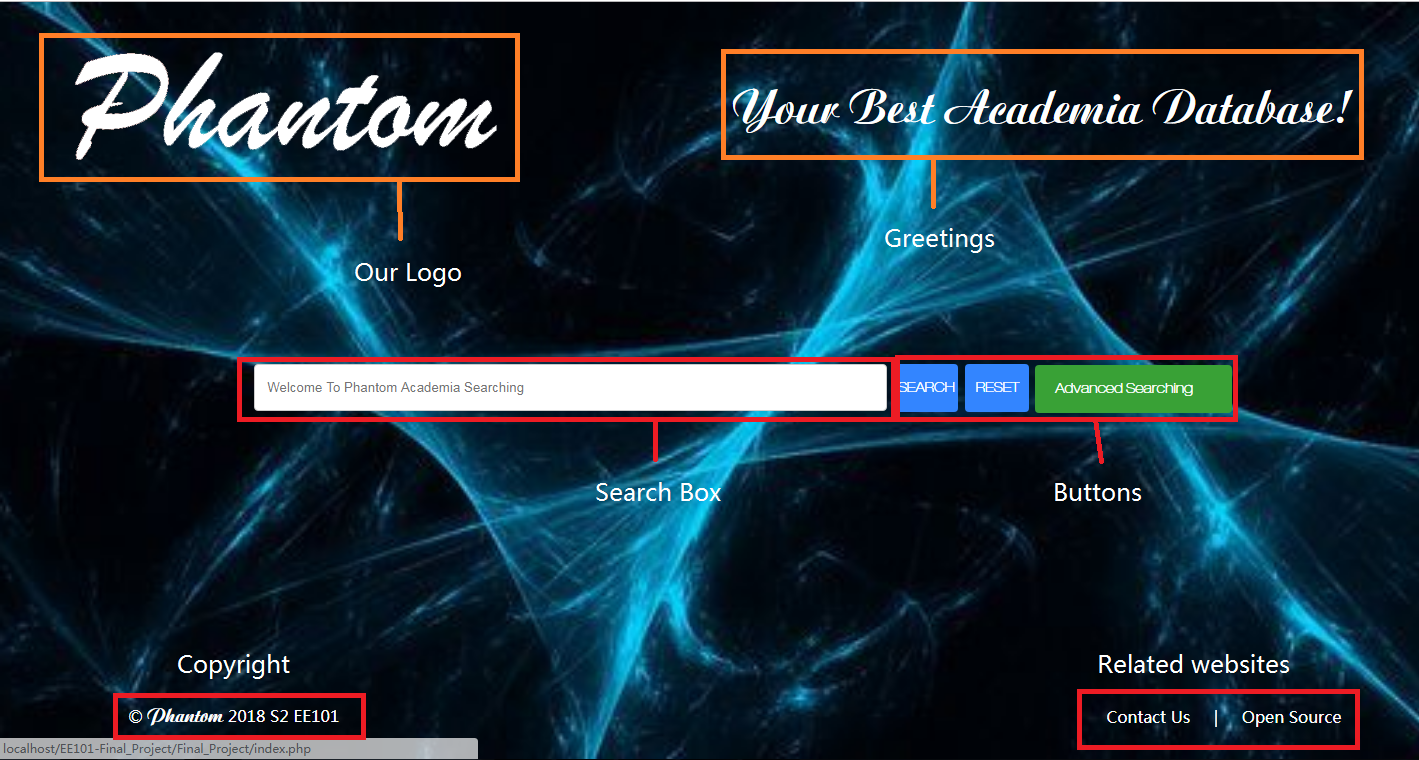
\includegraphics[width=0.7\textwidth]{cyf/index_structure.PNG}
	
	Our index page is shown above.First of all,I would like to introduce the process of my designing our home page.At first,there were three search boxes in the page.The search box "Author","Title" and "conference",and the layout of the index.php was settled.Then,we decided to use multi-searching.Therefore I cut down the number of search boxes into one.Finally,I polished the index.php and the page became what you can see now.
	
	The elements the index page consists of was shown in the graph above,ang I am going to introduce every part respectively.
	
	\subsubsection{Logo}
	
	The name of our search engine came from \emph{The Phantom of the opera},one of my favorite films,and I hope that the speed of our searching engine can be as fast as a phantom.It took me so much time to find a appropriate font to display our logo.Finally I found out a font "书体坊兰亭体".However,the words could not be shown in terms of vector graph,which meant that the edge of the words were not smooth,and that is a defect a our logo.
	
	\subsubsection{Greeting Words}
	
	To display the greeting words,I also spent plenty of time to find a approriate fonts.Finally, I found a font named "ChannelSlanted2" to present the greeting words.
	
	\subsubsection{Search box \& buttons}
	
	The search box and the buttons are the key part of the page,and I beautified the buttons,and the result was shown in the following pictures.
	\newline
	\newline
	
\includegraphics[width=0.7\textwidth]{cyf/search1.png}
	\newline
	
\includegraphics[width=0.7\textwidth]{cyf/search2.png}
	\newline
 	
\includegraphics[width=0.7\textwidth]{cyf/search3.png}
 	\newline	
 	
\includegraphics[width=0.7\textwidth]{cyf/search4.png}
 	\newline	
\includegraphics[width=0.7\textwidth]{cyf/search5.png}
 	\newline	
\includegraphics[width=0.7\textwidth]{cyf/search6.png}
 	\newline	
\includegraphics[width=0.7\textwidth]{cyf/search7.png}
 	\newline
	
\includegraphics[width=0.7\textwidth]{cyf/reset1.png}
	\newline
	
\includegraphics[width=0.7\textwidth]{cyf/reset2.png}
	\newline
	
\includegraphics[width=0.7\textwidth]{cyf/reset3.png}
	\newline	
	
\includegraphics[width=0.7\textwidth]{cyf/reset4.png}
	\newline	
\includegraphics[width=0.7\textwidth]{cyf/reset5.png}
	\newline	
\includegraphics[width=0.7\textwidth]{cyf/reset6.png}
	\newline	
\includegraphics[width=0.7\textwidth]{cyf/reset7.png}
	\newline
	
\includegraphics[width=0.7\textwidth]{cyf/Advanced_searching1.png}
	\newline
	
\includegraphics[width=0.7\textwidth]{cyf/Advanced_searching2.png}
	\newline
	
\includegraphics[width=0.7\textwidth]{cyf/Advanced_searching3.png}
	\newline	
	
\includegraphics[width=0.7\textwidth]{cyf/Advanced_searching4.png}
	\newline	
\includegraphics[width=0.7\textwidth]{cyf/Advanced_searching5.png}
	\newline	
\includegraphics[width=0.7\textwidth]{cyf/Advanced_searching6.png}
	\newline	
\includegraphics[width=0.7\textwidth]{cyf/Advanced_searching7.png}
	\newline
	
\includegraphics[width=0.7\textwidth]{cyf/Advanced_searching8.png}
	\newline
	
\includegraphics[width=0.7\textwidth]{cyf/Advanced_searching9.png}
	\newline
	
\includegraphics[width=0.7\textwidth]{cyf/Advanced_searching10.png}
	\newline	
	
\includegraphics[width=0.7\textwidth]{cyf/Advanced_searching11.png}
	\newline	
\includegraphics[width=0.7\textwidth]{cyf/Advanced_searching12.png}
	\newline	
\includegraphics[width=0.7\textwidth]{cyf/Advanced_searching13.png}
	\newline	
\includegraphics[width=0.7\textwidth]{cyf/Advanced_searching14.png}
	\newline	
\includegraphics[width=0.7\textwidth]{cyf/Advanced_searching15.png}
	\newline	
\includegraphics[width=0.7\textwidth]{cyf/Advanced_searching16.png}
	\newline	
\includegraphics[width=0.7\textwidth]{cyf/Advanced_searching17.png}
	\newline	
\includegraphics[width=0.7\textwidth]{cyf/Advanced_searching18.png}
	\newline	
\includegraphics[width=0.7\textwidth]{cyf/Advanced_searching19.png}
	\newline	
\includegraphics[width=0.7\textwidth]{cyf/Advanced_searching20.png}
	\newline	
\includegraphics[width=0.7\textwidth]{cyf/Advanced_searching21.png}
	\newline	
\includegraphics[width=0.7\textwidth]{cyf/Advanced_searching22.png}
	\newline	
\includegraphics[width=0.7\textwidth]{cyf/Advanced_searching23.png}
	\newline	
\includegraphics[width=0.7\textwidth]{cyf/Advanced_searching24.png}
	\newline	
\includegraphics[width=0.7\textwidth]{cyf/Advanced_searching25.png}
	\newline	
\includegraphics[width=0.7\textwidth]{cyf/Advanced_searching26.png}
	\newline	
\includegraphics[width=0.7\textwidth]{cyf/Advanced_searching27.png}
	\newline	
\includegraphics[width=0.7\textwidth]{cyf/Advanced_searching28.png}
	\newline	
\includegraphics[width=0.7\textwidth]{cyf/Advanced_searching29.png}
	\newline	
\includegraphics[width=0.7\textwidth]{cyf/Advanced_searching30.png}
	\newline	
\includegraphics[width=0.7\textwidth]{cyf/Advanced_searching31.png}
	
	\subsubsection{Copyright \& Related Websites}
	
	These two parts were mainly written by Ziliang Guo and Aofan Jiang and Hyperlinks were set on the texts "Contact Us" and "Open source".
	
	\subsection{Search}
		
	
	 
	
	
	

\end{document}